\documentclass[11pt,a4paper]{article}
\usepackage{tikz}
\usepackage[left=2cm,right=2cm,top=2cm,bottom=2.3cm]{geometry}
\usepackage{amssymb,amsmath}
\usepackage[unicode,colorlinks]{hyperref}
\usepackage{wrapfig}

\usepackage[utf8]{input enc}
\usepackage[english, russian]{babel}

\newcommand{\nn}{\nonumber}
\newcommand{\pt}{\partial}
\newcommand{\grad}{\mathrm{grad}\,}
\newcommand{\rot}{\mathrm{rot}\,}
\renewcommand{\div}{\mathrm{div}\,}
\newcommand{\vn}{\vec{\nabla}}

\title{Электродинамика}
\author{Игорь Шендерович\\\texttt{shender.i@gmail.com}}
\begin{document}
\maketitle

\section{Векторные поля. Основные определения. Аналогия с гидродинамикой.}

Рассмотрим электрический заряд $q$, расположенный в какой-нибудь точке
в пространстве. Этот заряд создаёт статическое электрическое поле. По
закону Кулона его напряжённость выражается формулой
\begin{equation}
  \label{eq:coulomb}
  \vec{E}(\vec{r}) = \frac{q \vec{r}}{r^3}.
\end{equation}

Видно, что вектор $\vec{E}$ существует в любой точке пространства, вне
зависимости от того, насколько далеко мы отошли от заряда. Это
позволяет ввести понятие \textit{векторного поля} --- вида материи,
который существует при наличии источника. В данном случае источником
электрического поля является заряд $q$. Позднее мы увидим, что
магнитное поле, несмотря на отсутсвие одиночных источников, также
допускает такую интерпретацию. С этого момента мы будем говорить не о
напряжённости $\vec{E}$, а об электрическом (или магнитном) поле
$\vec{E}(x,y,z,t)$ (или $\vec{B}(x,y,z,t)$). Заметим, что поле может
зависеть как от точки пространства, так и от времени. 

Поскольку вектор определяется своими проекциями, то задать векторное
поле --- то же самое, что задать три его проекции. Таким образом,
электрическое поле $\vec{E}$ --- три функции четырёх переменных. 

Понятно, что в природе существуют и другие поля, не обязательно
векторные. Рассмотрим, например, поле температур $T(x,y,z,t)$. Это
тоже поле (т.к. температуру можно определить в любой точке
пространства), но \textit{скалярное}, поскольку температура не имеет
направления, а определяется лишь числовым значением. 

Другой пример векторного поля, более приближенный к реальности ---
поле скоростей жидкости. Каждой <<частице>> движущейся жидкости можно
сопоставить векторную функцию $\vec{v}(\vec{r},t)$, которая описывает
скорость данной частички. По определению, это векторное поле
скоростей. Мы увидим в дальнейшем, что многие свойства этого поля
жидкости переносятся и на электродинамику. 

Электрические и магнитные (или просто электромагнитные) поля устроены
довольно сложно, но при этом связь между значениями полей в двух
соседних точках довольно проста. Задача наших упражнений --- вывести
эту связь в наиболее общем виде. 

\begin{wrapfigure}{r}{40mm}
  \vspace{-1cm}
  \begin{center}
  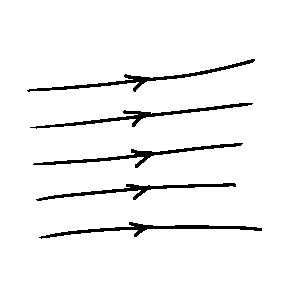
\includegraphics[width=4cm]{pics/lines.pdf}  
  \end{center}
  \vspace{-1cm}
  \caption{Силовые линии.}
  \label{fig:force_lines}
  \vspace{-1.1cm}
\end{wrapfigure}

Как можно зрительно представлять поля? Лучше всего это делать с
помощью \emph{силовых линий} --- таких линий, касательные к которым в
каждой точке будут давать направление вектора напряжённости в этой
точке. 

Чтобы изобразить на подобной картинке величину модуля вектора
напряжённости, можно условиться рисовать линии гуще в тех местах, где
абсолютная величина этого вектора больше. 

\subsection{Поток.}
\label{sec:flux}

Векторные поля обладают двумя очень важными характеристиками, которые
мы будем использовать при описании. Первая из них --- \emph{поток}. 

Рассмотрим, к примеру, поток жидкости через некоторую ограниченную
поверхность. Можно задать себе вопрос --- сколько жидкости втекает
(вытекает) через эту поверхность площади $S$? 

Это количество можно посчитать следующим образом. Разобъём нашу
поверхность на много кусочков с площадью $dS$ каждый. К каждому
кусочку проведём вектор нормали $\vec{n}$ (так, чтобы он смотрел
наружу поверхности, а не внутрь). Тем самым, у каждого кусочка площади
будет задана ориентация. Для краткости совокупность данных о площади
кусочка и векторе нормали можно записывать в виде одного вектора
$d\vec{S}$ --- это вектор, по модулю равный $dS$, с направлением,
совпадающим с $\vec{n}$.

\begin{wrapfigure}{r}{40mm}
  \vspace{-1cm}
  \begin{center}
    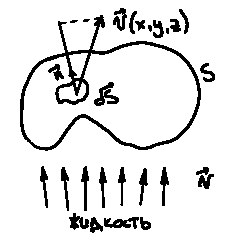
\includegraphics[width=4cm,height=4cm]{pics/flux.pdf}
  \end{center}
  \vspace{-0.7cm}
  \caption{Поток.}
  \label{fig:flux}
\end{wrapfigure}

Спроецируем на направление этого вектора наше поле $\vec{v}$. Операция
проектирования проще всего выглядит как скалярное произведение
$\vec{v} \cdot d \vec{S}$. Действительно, по определению, скалярное
произведение равно $d\Phi = v \cdot dS \cdot \cos \alpha$, где $\alpha$ ---
угол между вектором $\vec{v}$ и нормалью $\vec{n}$. Теперь
просуммируем подобные выражения по всей поверхности, иными словами,
проинтегрируем по ней:

\begin{equation}
  \label{eq:def_flux}
  \Phi \equiv \int_S \vec{v} \cdot d \vec{S}.
\end{equation}

По определению, это скалярное произведение и называется потоком $\Phi$ 
векторного поля $\vec{v}$. Можно интерпретировать это определение и
таким способом: поток векторного поля равен среднему значению
нормальной компоненты поля $\vec{v}$, умноженному на величину площади
$S$. 

Если, например, поле устроено так, что не зависит от конкретной точки
(всюду постоянное поле), то формула для расчёта потока может быть
сильно упрощена. Пусть, скажем, поле всюду направлено по нормали к
поверхности (пример --- электрическое поле точечного заряда, а
поверхность --- сфера). Тогда в любой точке скалярное произведение
превращается в обычное (т.к. $\cos 0 = 1$), и функцию $v$ можно
вынести за знак интеграла. Интеграл же от $dS$ даст просто площадь
поверхности. Таким образом, в этом простейшем случае поток станет
равен $\Phi = vS$. 

В более сложных случаях (которые обычно и встречаются в природе),
вычисление потока по определению --- довольно сложная задача. К
счастью, у нас будет \emph{теорема Гаусса}, которая позволяет свести
вычисление потока к относительно простым операциям. 

\subsection{Циркуляция.}
\label{sec:curl}

Опять представим себе поле скоростей, описывающее поток
жидкости. Зададимся таким вопросом: циркулирует ли эта жидкость? Иными
словами, существует ли её вращательное движение вдоль некоторого
замкнутого геометрического контура? 

\begin{wrapfigure}{r}{40mm}
  \vspace{-1.5cm}
  \begin{center}
    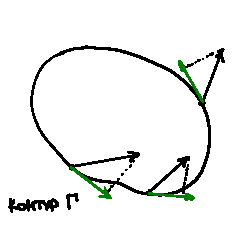
\includegraphics[width=4cm,height=4cm]{pics/curl.pdf}
  \end{center}
  \vspace{-0.7cm}
  \caption{Циркуляция.}
  \label{fig:curl}
\end{wrapfigure}


По определению, \emph{циркуляцией} $C$ называется скорость жидкости вдоль
контура, умноженная на длину этого контура. Как и в случае с потоком,
можно думать про эти величины как про средние; более аккуратное
определение можно получить, опять пользуясь понятием проекции. 

Рассмотрим участок контура длиной $dl$. С ним, как и с кусочком
площадки, можно связать направление. Рассмотрим вектор $d\vec{l}$ ---
это вектор, модуль которого равен $dl$, а направление совпадает с
направлением касательной в данной точке. Теперь спроецируем наше
векторное поле $\vec{v}$ на этот вектор $d\vec{l}$. Сделать это можно
так же, как и в случае с потоком, т.е. взять скалярное
произведение. Теперь просуммируем это по всему контуру:

\begin{equation}
  \label{eq:curl}
  C \equiv \oint_\Gamma \vec{v} \cdot d \vec{l}.
\end{equation}

Пользуясь понятиями потока и циркуляции, мы опишем все законы
электродинамики, т.е. получим уравнения Максвелла. 

\subsection{Операции векторного анализа.}
\label{sec:vector_analysis}

Разберём подробнее операции с векторами. Нам понадобится умение
перемножать вектора двумя способами, дифференцировать их и
интегрировать. 

\subsubsection{Произведения векторов. }

Два вектора $\vec{a}$ и $\vec{b}$ можно перемножить двумя способами:
скалярно и векторно. \emph{Скалярное произведение} определяется через
компоненты этих векторов:

\begin{equation}
  \label{eq:def_scalar_product}
  \vec{a} \cdot \vec{b} \equiv a_x b_x + a_y b_y + a_z b_z.
\end{equation}

С помощью скалярного произведения можно также определить модуль
вектора: это корень из скалярного произведения вектора на самого себя.

\begin{equation}
  \label{eq:def_modulus_vector}
  |a| \equiv \sqrt{\vec{a} \cdot \vec{a}}.
\end{equation}

Также можно образовать \emph{векторное произведение}: такое
произведение двух векторов, результатом которого является снова
вектор. Модуль этого вектора равен

\begin{equation}
  \label{eq:def_cross_product}
  | \vec{a} \times \vec{b}| = |\vec{a}| |\vec{b}| \sin \alpha,  
\end{equation}
а направление задаётся правилом правой руки. Угол $\alpha$ --- угол
между векторами. 

\begin{wrapfigure}{r}{40mm}
  \vspace{-1.5cm}
  \begin{center}
    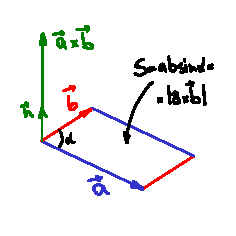
\includegraphics[width=4cm,height=4cm]{pics/cross.pdf}
  \end{center}
  \vspace{-0.7cm}
  \caption{Векторное произведение.}
  \label{fig:curl}
  \vspace{-1cm}
\end{wrapfigure}

Свойства этого произведения довольно просты. Во-первых, если вектора
$\vec{a}$ и $\vec{b}$ коллинеарны, то $\vec{a} \times
\vec{b}=0$. Во-вторых, модуль этого вектора совпадает с площадью
параллелограмма, натянутого на вектора $\vec{a}$ и $\vec{b}$.

А можно ли записать определение векторного произведения в координатах,
подобно \eqref{eq:def_scalar_product}? Оказывается, можно. Именно, 

\begin{eqnarray}
  \label{eq:def_cross_product_components}
  \nn
  (\vec{a} \times \vec{b})_x &=& a_y b_z -a_z b_y,\\
  (\vec{a} \times \vec{b})_y &=& a_z b_x -a_x b_z,\\
  \nn
  (\vec{a} \times \vec{b})_z &=& a_x b_y -a_y b_x.
\end{eqnarray}

Запомнить это правило довольно просто: для i-ой компоненты нужно
устроить циклическую перестановку из индексов (xyz), где нужный индекс
стоит на i-ом месте. 

Понять, откуда взялось это правило, довольно просто. Рассмотрим три
орта $\vec{i},\vec{j},\vec{k}$. Применяя к ним правило
\eqref{eq:def_cross_product}, получим, что $\vec{i} \times \vec{j} =
\vec{k}$, \ldots. Расписывая вектор $\vec{a} = a_x \vec{i} + a_y
\vec{j} + a_z \vec{k}$, а вектор $\vec{b}$ аналогично, получим
требуемые свойства \eqref{eq:def_cross_product_components}. 

\subsection{Градиент. Оператор $\nabla$.}
\label{sec:gradient}

Предположим, что у нас имеется для начала скалярное поле, типа поля
температур. Мы хотим как-то описать изменение температуры $T(x,y,z,t)$
в пространстве. В отличие от похожей задачи --- изменения температуры
по времени --- нам нужно дифференцировать не по времени, а придумать
что-то другое, более подходящее к данному случаю.

Понятно, что если бы у нас была одна координата, то сработала бы
производная $dT/dx$, потому что именно она бы определяла скорость
изменения температуры вдоль оси $x$. В данном случае нам понадобятся
три производных 

\begin{equation}
  \label{eq:def_grad_1}
  \frac{\pt T}{\pt x}, \quad   \frac{\pt T}{\pt y}, \quad   \frac{\pt
    T}{\pt z},
\end{equation}
из которых можно сделать вектор. Вектор можно соорудить естественным
способом. Вспомним, что у нас есть три орта
$\vec{i},\vec{j},\vec{k}$. Построим вектор \emph{градиента} по такому
правилу:

\begin{equation}
  \label{eq:def_grad_2}
  \grad T (x,y,z) \equiv \nabla T \equiv \frac{\pt T}{\pt x} \vec{i} +  \frac{\pt T}{\pt y}
  \vec{j} +  \frac{\pt T}{\pt z} \vec{k}.
\end{equation}

Таким образом, можно сказать, что градиент скалярного поля --- это
аналог производной, только в числе измерений больше одного. 

Заметим, что градиент, будучи вектором, явно зависит от
направления. Это сооветствует тому факту, что температура в разных
направлениях пространства может вестии себя по-разному. Таким образом,
градиент температуры $\grad T$ --- векторное поле, образованное из скалярного
поля самой температуры $T$.

Физический смысл градиента такой: в каждой точке пространства он
указывает направление, в котором температура меняется быстрее всего. 

Оказывается, что у градиента есть ещё одна интерпретация. Она ведёт к
обобщению известной теоремы \emph{Ньютона--Лейбница}. Эта теорема
устроена примерно так. Представим себе, что у нас есть материальная
точка, двигающаяся в пространстве. Её координаты мы будем
характеризовать радиус--вектором $\vec{r}(t)$. Вычислим скорость этой
материальной точки; по определению, она равна $\vec{v} (t) = d
\vec{r}(t) / dt$. Что получится, если мы теперь проинтегрируем эту
скорость по времени от момента $t_1$ до $t_2$? 

\begin{equation}
  \label{eq:newton_leibnitz}
  \int_{t_1}^{t_2} \vec{v}(t) \, dt = \int_{t_1}^{t_2}
  \frac{d\vec{r}(t)} {dt} \, dt = \int_{t_1}^{t_2} d\vec{r}(t) =
  \vec{r}(t_2) - \vec{r}(t_1) = \Delta \vec{r}.
\end{equation}

То есть, если проинтегрировать скорость, получится перемещение. Более
общо: если проинтегрировать производную некоторой функции $f(t)$,
получится изменение этой самой функции $f(t)$. 

Эта теорема естественным образом ограничена на прямую линию (интеграл
вдоль прямой). Что будет, если мы захотим проинтегрировать что-нибудь
(а точнее, какой--нибудь вектор) вдоль произвольной кривой? 

\begin{wrapfigure}{r}{40mm}
  \vspace{-1.2cm}
  \begin{center}
    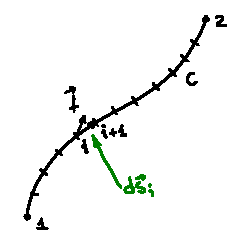
\includegraphics[width=4cm,height=4cm]{pics/curve_int.pdf}
  \end{center}
  \vspace{-0.7cm}
  \caption{Интеграл вдоль кривой.}
  \label{fig:curve_int}
\end{wrapfigure}


В этом случае нам нужно описать процедуру интегрирования вдоль
кривой. Рассмотрим кусочек дуги кривой $\Delta s_i$. Пускай значение функции
на нашем кусочке равно $f_i$. Тогда интегралом вдоль кривой $C$
называется такое выражение:

\begin{equation}
  \label{eq:def_curve_int_1}
  \int_C  \vec{f} \cdot d\vec{s} \equiv \lim_{N\to \infty} \sum_{i=0}^N f_i \Delta s_i. 
\end{equation}

В общем, это что-то, аналогичное стандартному определению интеграла,
только нужно учитывать, что $f_i$ --- значение функции на этом
отрезке. В нашем случае вместо скаляра $f_i$ уместно взять скалярное
произведение 

\begin{equation}
  \label{eq:def_curve_int_2}
  \grad \phi \cdot d\vec{s}_i.
\end{equation}

Мы уже знаем, что градиент показывает, насколько быстро меняется
функция в данном направлении. Таким образом, если мы спроецируем
градиент на какое-то выделенное направление, мы получим скорость
изменения функции в этом направлении. Проецирование делатся в точности
скалярным произведением \eqref{eq:def_curve_int_2}. Таким образом,
уравнение \eqref{eq:def_curve_int_2} даёт изменение скалярного поля в
направлении $d\vec{s}_i = \phi(i+1) - \phi(i)$, где $\phi(i)$ ---
значение поля в точке $i$. Суммируя все такие изменения, получаем, что
сумма \eqref{eq:def_curve_int_1} превращается в конечное изменение 

\begin{equation}
  \label{eq:def_curve_int_3}
  \int_C \grad \phi \cdot d\vec{s} = \phi(2) - \phi(1).
\end{equation}

Таким образом, мы видим, что у градиента есть такой смысл: будучи
проинтегрирован по какой-либо кривой, он даёт изменение конечное
изменение скалярной функции вдоль этой кривой. 

Заметим попутно, что интеграл от градиента, очевидно, не зависит от
кривой, вдоль которой мы интегрируем. Действительно, правая часть
уравнения \eqref{eq:def_curve_int_3} зависит только от значений поля
$\phi$ в точках 1 и 2, и больше не от чего. Очевидно, что значения
поля в этих точках не зависят от того, по какому пути мы в эти точки
пришли. 

Что будет, если мы придём из точки 1 в точку 2 по красному пути, а
уйдём обратно по синему? Мы опишем замкнутый контур. 

\begin{wrapfigure}{r}{40mm}
  \vspace{-1.5cm}
  \begin{center}
    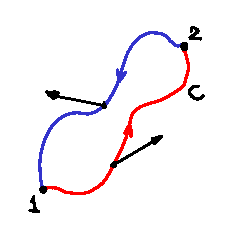
\includegraphics[width=4cm,height=4cm]{pics/path_indep.pdf}
  \end{center}
  \vspace{-0.7cm}
  \caption{Замкнутый контур.}
  \label{fig:path_indep}
\end{wrapfigure}

Пройдём по красному контуру от точки 1 до точки 2. При этом значение
интеграла \eqref{eq:def_curve_int_3} даст нам, как и положено, $\phi(2)
- \phi(1)$. Теперь пройдём от точки 2 до точки 1 по синему
контуру. Интеграл даст на этот раз $\phi(1) - \phi(2)$. В итоге наших
прогулок по разноцветным контурам мы придём обратно в точку 1, при
этом значение интеграла по замкнутому контуру будет равно 0. Опять же,
заметим, что он конкретной формы этого контура ничего не зависит. 

Таким образом, мы доказали, что интеграл от градиента по замкнутому
контуру равен нулю, и от контура не зависит. Или, вспоминая
определение циркуляции \eqref{eq:curl}, мы доказали, что циркуляция
градиента равна нулю.

\begin{equation}
  \label{eq:int_grad}
  \oint \grad \phi \cdot  d\vec{l} =0.
\end{equation}

В дальнейшем этот факт нам поможет. 

Напоследок продемонстрируем один трюк, ради которого (отчасти) это всё
и затевалось. Обозначим \emph{формально} буквой $\nabla$ такую
операцию:

\begin{equation}
  \label{eq:def_nabla}
  \vec{\nabla} \equiv \frac{\pt}{\pt x} \vec{i} +  \frac{\pt}{\pt y}
  \vec{j} +  \frac{\pt}{\pt z} \vec{k}.
\end{equation}

Буква $\vec{\nabla}$ теперь играет роль \emph{оператора градиента},
т.е. не самостоятельной буквы, а чего-то, что имеет смысл только в
паре с функцией, к которой она применяется. Оператор градиента
<<ждёт>> функцию, которую ему надо продифференцировать. Из формулы
\eqref{eq:def_grad_2} видно, что градиент можно получить, действуя
оператором градиента на наше скалярное поле.

Очевидно, что, будучи вектором, оператор $\vec{\nabla}$ может быть применён
не только к скалярам (типа поля температуры), но и к векторам,
порождая объекты с очень прозрачным физическим смыслом. 

\subsection{Дивергенция.}
\label{sec:divergence}

Первое, что мы можем сделать с вектором $\vec{\nabla}$ и каким-то
векторным полем $\vec{A}$ --- скалярно их перемножить. Как следует из
определения, должен получиться скаляр. Посмотрим, так ли это.

\begin{equation}
  \label{eq:def_divergence}
  \div \vec{A} \equiv \vec{\nabla} \cdot \vec{A} = \frac{\pt}{\pt x}
  A_x +  \frac{\pt}{\pt y} A_y +  \frac{\pt}{\pt z} A_z = \frac{\pt
    A_x}{\pt x} +  \frac{\pt A_y}{\pt y} +  \frac{\pt A_z}{\pt z}.
\end{equation}

Скалярная величина, которую мы получили, называется
\emph{дивергенцией}. Фактически, оператор $\vec{\nabla}$, скалярно
умноженный на $\vec{A}$, дифференцирует каждую из компонент вектора
$\vec{A}$ по соответствующей координате и складывает результаты без
учёта направления. Этим он и отличается от градиента: градиент,
напомним, даёт вектор. 

Итак, если градиент скалярному полю сопоставляет векторное, то
дивергенция векторному полю сопоставляет скалярное. 

Нет ли случайно у дивергенции какого-нибудь внятного физического
смысла? Разумеется, есть, иначе зачем бы она нам понадобилась!

Чтобы понять этот физический смысл, нам понадобится вспомнить понятие
потока \eqref{eq:def_flux}. Именно, рассмотрим маленький кубик со
сторонами $\Delta x$, $\Delta y$, $\Delta z$. Пускай в пространстве есть какое-то
векторное поле $\vec{A}$. Вычислим его поток (наружу) через
поверхность этого кубика.

У поверхности кубика 6 граней. Можно вычислить поток через каждую из
них. Поскольку грани --- маленькие квадраты, вычисление будет
несложным. Например, поток через грань 1 равен

\begin{equation}
  \label{eq:theorem_divergence_1}
  \Phi_1 = -\int A_y (x,y,z) dx dz.
\end{equation}
(знак минус появился от того, что в грань 1 наше поле \emph{входит},
так что поток \emph{наружу} будет со знаком минус). Это выражение
можно упростить: так как мы считаем наш кубик маленьким, то можно
считать, что на грани функция $A_y$ примерно постоянная; раз так, то
её можно вытащить за знак интеграла. Останется лишь интеграл по
площади грани, который равен собственно площади $\Delta x \Delta z$. 

\begin{wrapfigure}{r}{40mm}
  \vspace{-1.2cm}
  \begin{center}
    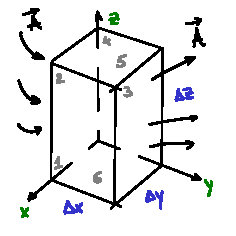
\includegraphics[width=4cm,height=4cm]{pics/div.pdf}
  \end{center}
  \vspace{-0.7cm}
  \caption{Вычисление потока.}
  \label{fig:div}
  \vspace{2cm}
\end{wrapfigure}

Итого, получаем, что поток через грань 1 равен

\begin{equation}
  \Phi_1 = - A_y \Delta x \Delta z. 
\end{equation}

Рассмотрим теперь поток наружу через грань 3:

\begin{equation}
  \Phi_3 = \int A_y (x,y + \Delta y,z) dx dz = A_y (x,y+\Delta y,z)
  \Delta x \Delta z.
\end{equation}

Сложим теперь потоки $\Phi_1 + \Phi_3$ --- это логично сделать, потому
что у них есть много общего. 

\begin{equation}
  \label{eq:theorem_divergence_2}
  \Phi_1 + \Phi_3 = \Delta x \Delta z \left(A_y(y+\Delta y) - A_y
    (y)\right) \approx \Delta x \Delta z \Delta y \frac{\pt A_y}{\pt y}.
\end{equation}

Здесь мы заменили разность полей на двух гранях производной потому,
что кубик считается маленьким и такая замена не внесёт существенной
ошибки. Аналогичные операции можно провернуть и для остальных четырёх
граней; ответ для полного потока $\Phi$ совсем не удивителен:

\begin{equation}
  \label{eq:theorem_divergence_3}
  \Phi = \Delta x \Delta y \Delta z
  \left(
    \frac{\pt A_x}{\pt x} + 
    \frac{\pt A_y}{\pt y} + 
    \frac{\pt A_z}{\pt z}
  \right) = \Delta V \div \vec{A}. 
\end{equation}

Таким образом, физический смысл дивергенции такой: это поток
векторного поля, отнесённый к единице объёма $\Delta V$. Можно
сказать, что дивергенция меряет <<удельную величину>> потока, измеряя,
насколько мощный источник поля мы имеем. 

\subsection{Ротор.}
\label{sec:curl}

Что ещё можно смастерить из оператора $\vec{\nabla}$ и вектора?
Помимо скалярного произведения, которое приводит к дивергенции, можно
сделать векторное произведение; в итоге получится вектор. Какие же у
него будут компоненты? Из формул \eqref{eq:def_cross_product} и
\eqref{eq:def_nabla} получаем: 

\begin{eqnarray}
  \label{eq:def_curl}
  \nn
  (\vec{\nabla} \times \vec{A})_x &=& \frac{\pt A_z}{\pt y} -  \frac{\pt
    A_y}{\pt z},\\
  (\vec{\nabla} \times \vec{A})_y &=& \frac{\pt A_x}{\pt z} -  \frac{\pt
    A_z}{\pt x},\\
  \nn
  (\vec{\nabla} \times \vec{A})_z &=& \frac{\pt A_y}{\pt x} -  \frac{\pt
    A_x}{\pt y}.
\end{eqnarray}

Вектор $\rot \vec{A} \equiv \vn \times \vec{A}$ называют
\emph{ротором} или \emph{вихрем}. Название выбрано неслучайно:
физический смысл этого вектора тесно связан с вихрями в потоке
жидкости (или в любом другом векторном поле).

Сейчас мы начнём получать дивиденды от записи векторных операций через
оператор $\vn$. Попробуем составить всякие комбинации с двумя
операторами $\vn$. Например, возьмём скалярное поле $\phi$, возьмём
его градиент (получится векторное поле), от получившегося сосчитаем
ротор. Кратко это записывается так:

\begin{equation}
  \vn \times (\vn \phi).
\end{equation}

Мы можем немедленно вычислить это произведение. Дело в том, что скобки
можно расставлять как угодно (произведение ассоциативно), поэтому
получаем, что $\vn \times (\vn \phi) = (\vn \times \vn) \phi
=0$. Здесь мы воспользовались тем, что векторное произведение вектора
самого на себя равно нулю (т.к. <<угол>> между векторами равен
нулю). Итак, мы получили следующее равенство: 

\begin{equation}
  \label{eq:rot_grad}
  \vn \times (\vn \phi) = \rot \grad \phi = 0.
\end{equation}

Рассмотрим теперь комбинацию $ \vec{A} \cdot (\vec{A} \times
\vec{B})$. Вектор $\vec{A} \times \vec{B}$ перпендикулярен $\vec{A}$
(см. рис. \ref{fig:curl}), поэтому это произведение равно
нулю. Возьмём теперь в качестве $\vec{A} = \vn$, а в качестве
$\vec{B}$ какое--нибудь векторное поле $\vec{V}$. Получаем

\begin{equation}
  \label{eq:div_rot}
  \vn \cdot (\vn \times \vec{V}) = 0 = \div \rot \vec{V}.
\end{equation}

Отметим, что эти соотношения верны для \textbf{любых} полей $\phi$ и
$\vec{V}$. Однако, не все соотношения с двумя операторами $\vn$ равны
нулю. К примеру, мы могли подействовать на градиент не ротором, а
дивергенцией:

\begin{equation}
  \label{eq:def_laplacian}
  \vn \cdot (\vn \phi) = \vn^2 \phi = \left( \frac{\pt^2}{\pt x^2} +
    \frac{\pt^2}{\pt y^2} + \frac{\pt^2}{\pt z^2} \right) \phi \equiv \Delta \phi.
\end{equation}

Оператор $\Delta$, встретившийся тут, называется \emph{лапласианом}. В
данном случае он переводит скалярное поле $\phi$ опять же в скаляр
(поскольку дивергенция --- скалярное поле). 

Раз оператор лапласиана скалярный, значит, он может действовать и на
вектор, т.е. на каждую компоненту вектора. 

\begin{equation}
  \vn^2 \vec{A} = \vn^2 A_x \vec{i} + \vn^2 A_y \vec{j} + \vn^2 A_z \vec{k}.
\end{equation}

\end{document}